\section{Aufbau}
\label{sec:Aufbau}

In Abbildung \ref{fig:Aufbau} ist ein schematischer Aufbau des Experiments zu sehen.
Der ganze Aufbau befindet sich in einer Vakuumkammer, die über eine Drehschieberpumpe betrieben wird und über ein Dosierventil belüftet werden kann.
Eine $^{241}.{Am}$-Probe wird in einer Halterung befestigt. Davor ist eine Kollimatorblende zur Fokussierung der $\alpha$-Teilchen angebracht.
Die Folie, die selbst auf einem Sockel mit Loch befestigt ist, kann auf einer beweglichen Drehscheibe angebracht werden, mit der die Folie aus dem Strahl gehoben werden kann, sodass dieser durch das Loch fällt.
Der Detektor kann auf einer Kreisbahn um die Folie herum bewegt werden und ist ebenfalls über eine Blende abgeschirmt wird.
Er kann entweder direkt oder über einen Verstärker an ein Oszilloskop angeschlossen oder über den Verstärker mit einem zeitgesteuerten Zähler verbunden werden.

\begin{figure}
\centering
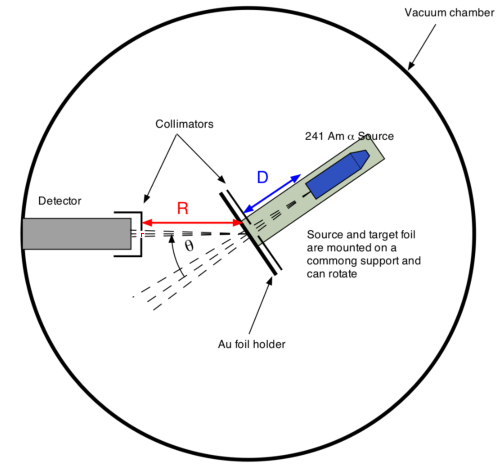
\includegraphics[width=\linewidth-70pt,keepaspectratio]{content/images/Aufbau2.pdf}
\caption{Schematischer Aufbau des Rutherford'schen Streuversuchs \cite{Aufbau16}.
Dabei ist $D=\SI{39}{\milli\meter}$ der Abstand zwischen Quelle und Kollimatorblende, $R=\SI{101}{\milli\meter}$ der Abstand zwischen Folie und Detektorblende und $r=\SI{5}{\milli\meter}$ der Radius der Detektorblende \cite{V16}.}
\label{fig:Aufbau}
\end{figure}

%☺♣